\documentclass[11pt,letterpaper]{article}

% Load some basic packages that are useful to have
% and that should be part of any LaTeX installation.
%
% be able to include figures
\usepackage{graphicx}
% get nice colors
\usepackage{xcolor}

% change default font to Palatino (looks nicer!)
\usepackage{apjfonts}
\usepackage{courier}
% load some useful math symbols/fonts
\usepackage{latexsym,amsfonts,amsmath,amssymb}

% comfort package to easily set margins
\usepackage[top=1in, bottom=1in, left=1in, right=1in]{geometry}

% control some spacings
%
% spacing after a paragraph
\setlength{\parskip}{.15cm}
% indentation at the top of a new paragraph
\setlength{\parindent}{0.0cm}


\begin{document}

\begin{center}
\Large
{\bf Ay190 -- Worksheet 11} \\
\large
Xiangcheng Ma \\
Date: \today
\end{center}

\section*{Poisson Equation}
(1) The density profile of the given star is showed in Figure \ref{fig1}.

\begin{figure}[bth]
\centering
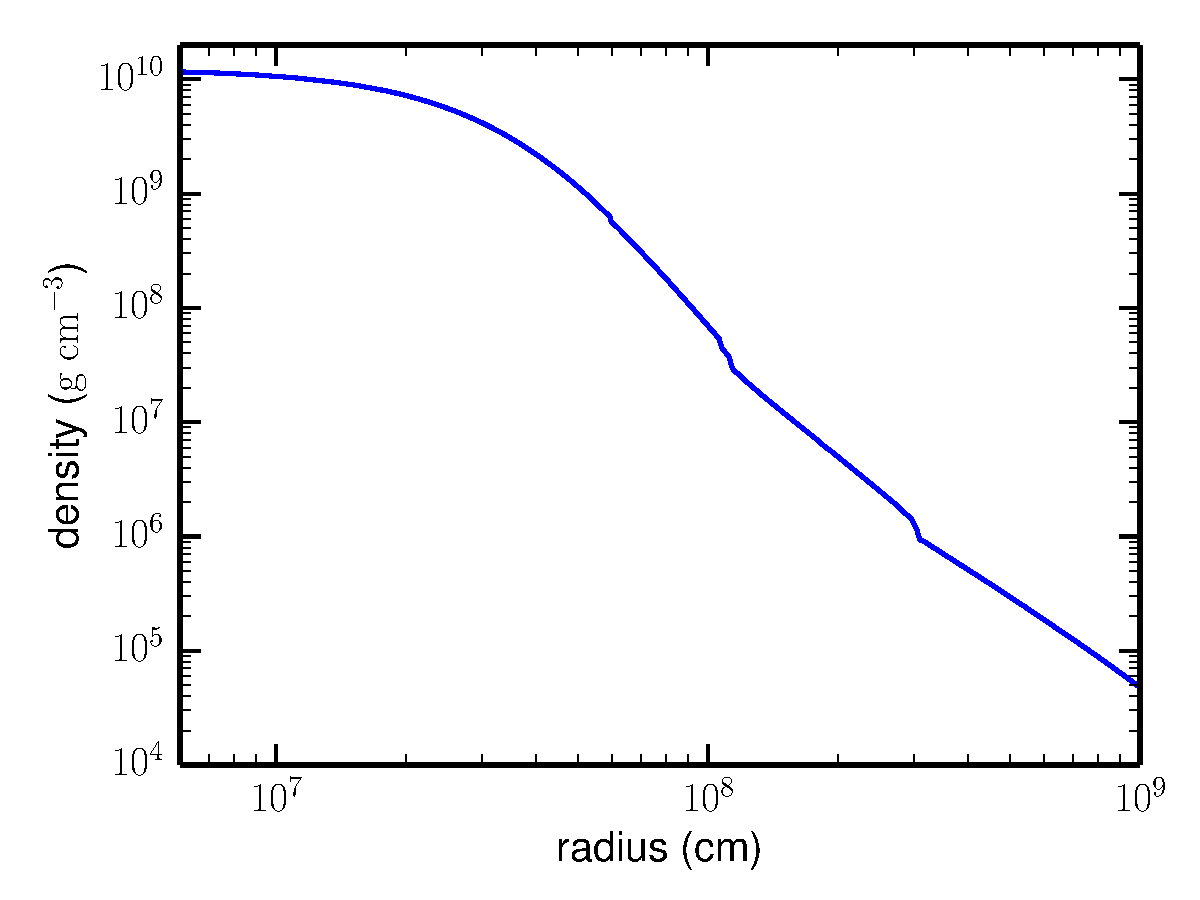
\includegraphics[width={0.8\textwidth}]{fig1.pdf} 
\caption{Density Profile}
\label{fig1}
\end{figure}

(2) The grid is set up from $6\times10^6$ cm to $10^9$ cm. I use the {\tt numpy.interp} routine to do the interpolation.

(3) A Euler intergrator has been implemented. I use a uniform density spread a radii from $0$ to $10^5$. The comparison is showed in Figure \ref{fig2}. The difference results in the error of Euler integration outward to the most outer radius. 

\begin{figure}[bth]
\centering
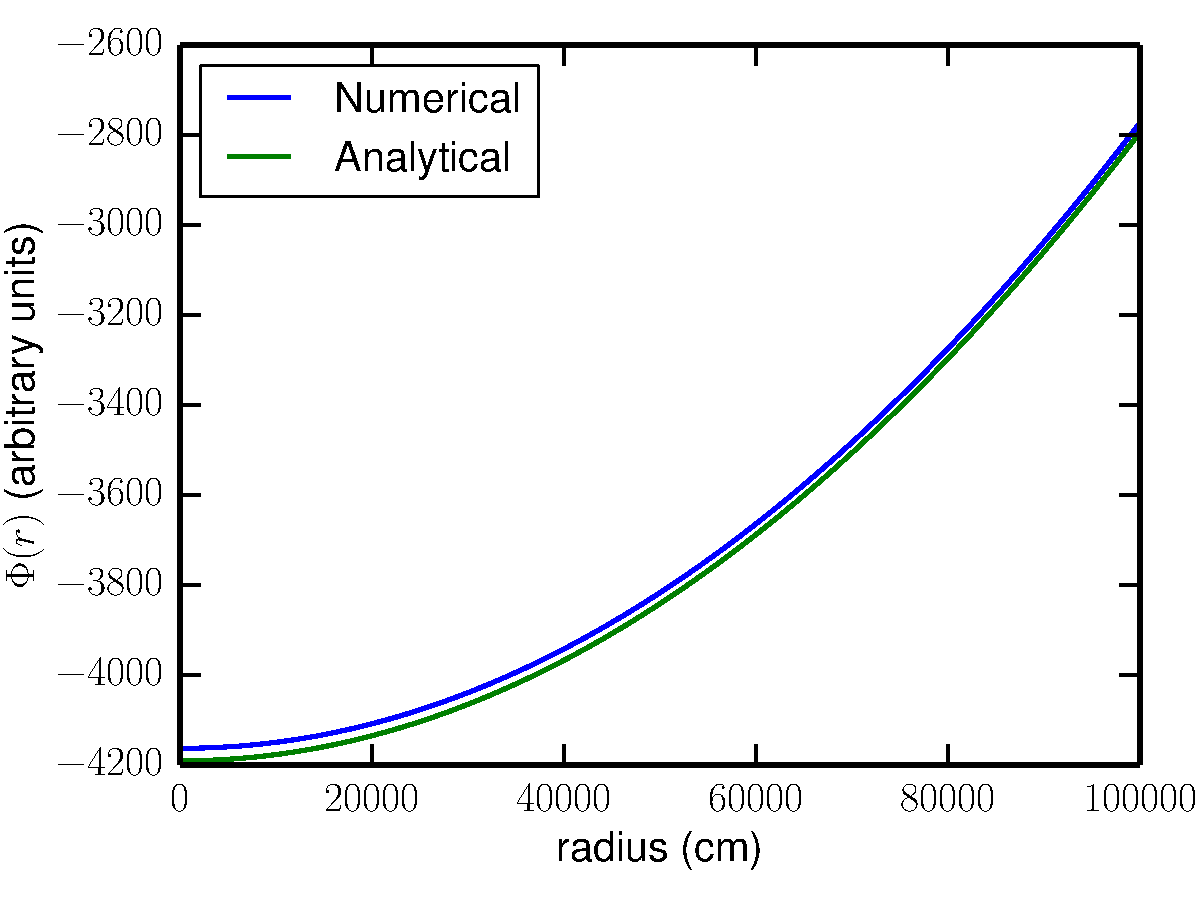
\includegraphics[width={0.8\textwidth}]{fig2.pdf} 
\caption{Uniform Density Test}
\label{fig2}
\end{figure}

The potential of the given star is plotted in Figure \ref{fig3}.

\begin{figure}[bth]
\centering
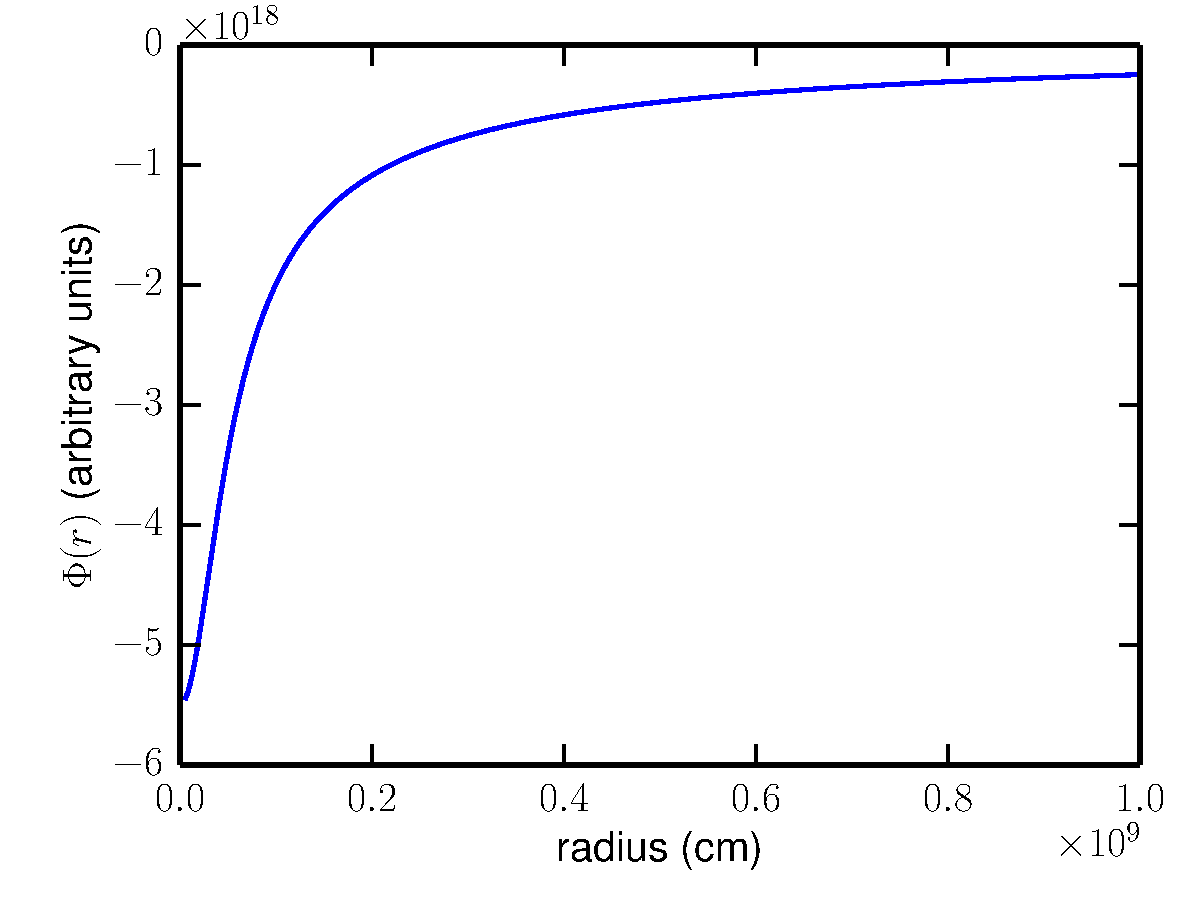
\includegraphics[width={0.8\textwidth}]{fig3.pdf} 
\caption{Potential of the Star}
\label{fig3}
\end{figure}

\end{document}
